
\documentclass{exam}

\usepackage{siunitx} 
\usepackage{graphicx}
\usepackage[fleqn]{amsmath}
\usepackage{cancel}
\usepackage{float}
\usepackage{mdwlist}
\usepackage{booktabs}
\usepackage{cancel}
\usepackage{polynom}
\usepackage{caption}
\usepackage{fullpage}

\newcommand{\degree}{\ensuremath{^\circ}} 
\everymath{\displaystyle}

% \begin{figure}[H]
%   \centering
%   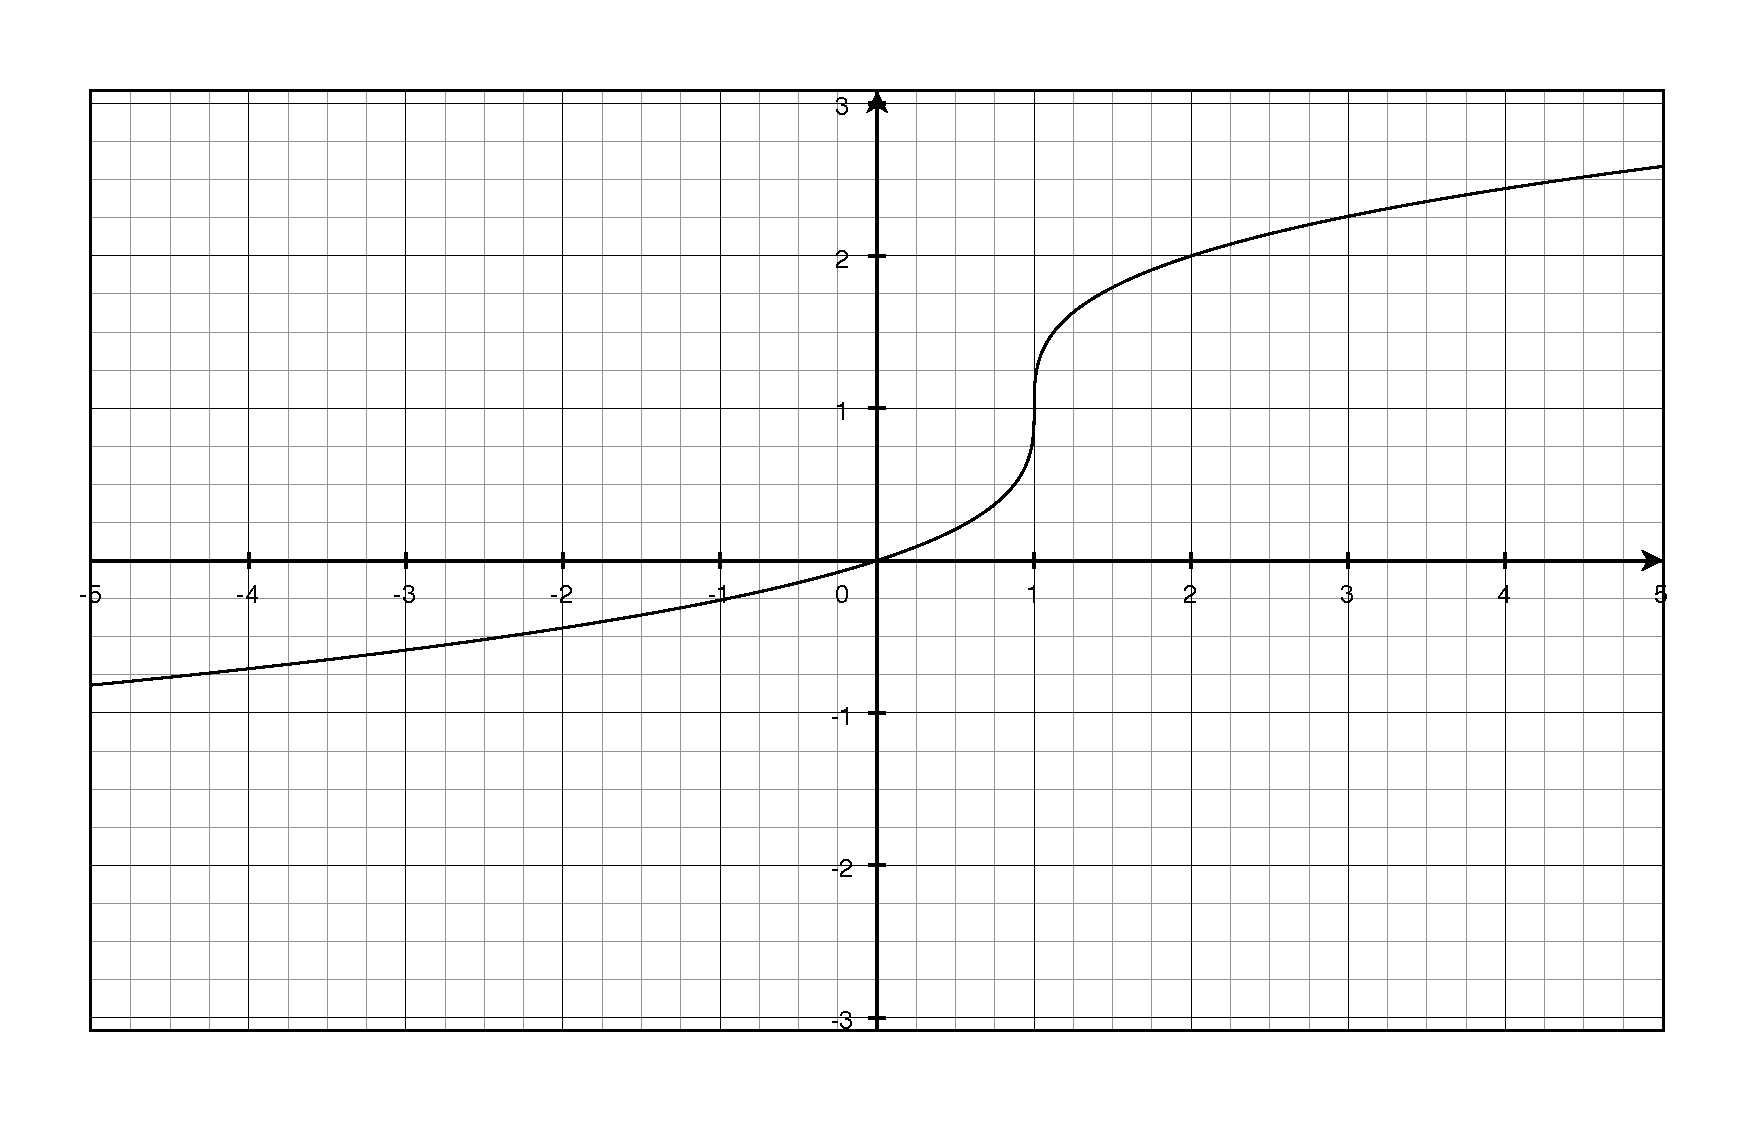
\includegraphics[scale=.3]{question7.eps}
%   \caption*{Question 7}
% \end{figure}

% \begin{tabular}{cc}
% \toprule
% period & amplitude \\
% \midrule
%   $\pi$ & $2$ \\
% \bottomrule
% \end{tabular}

\printanswers

\ifprintanswers 
\usepackage{2in1, lscape} 
\fi

\title{Math 263B \\ Homework One}
\date{July 12, 2012}

\begin{document}

\maketitle

\section{Homework}

\begin{itemize*}
  \item Read Section 5.1
  \item pp 237-238: 1-13, 17-18, 20-25, 27-30, 33-36
\end{itemize*}

\ifprintanswers
\pagebreak
\fi

\section{Extra Credit}
page 238, problem 48

\begin{solution}

Since $u = \sin[(x^2 + 1)^4]$, from the chain rule: 
\begin{align*}
  \frac{du}{dx} &= \cos \left[ \left( x^2 + 1 \right)^4 \right] \cdot 4 \left( x^2 + 1 \right) \cdot 2x \\
  du &= 8x \cdot \cos \left[ \left( x^2 + 1 \right)^4 \right] \cdot \left( x^2 + 1 \right) dx
\end{align*}

So we can rewrite the original problem as:
\[
  \int u^3 \frac{1}{8} \, \mathrm{d}u = \frac{1}{8} \int u^3 \, \mathrm{d}u = \frac{1}{32} u^4 + C
\]

And then plug $\sin \left[ \left( x^2 + 1 \right)^4 \right]$ back in for $u$:
\[
  \frac{1}{32} \sin^4 \left(x^2 + 1 \right)^4 + C
\]

\end{solution}

\ifprintanswers
\pagebreak

\begin{description}
\item[1]
\[
  \int 5 \, \mathrm{d}x = 5x + C \\
\]

\item[2]
\[
  \int (x - 4) \, \mathrm{d}x = \frac{1}{2} x^2 - 4x + C \\
\]

\item[3]
\[
  \int \left( x^2 + \pi \right)\, \mathrm{d}x = \frac{1}{3} x^3 + \pi x + C \\
\]

\item[4]
\[
  \int \left( 3x^2 + \sqrt{3} \right) \, \mathrm{d}x = x^3 + \sqrt{3} \cdot x + C \\
\]

\item[5]
\[
  \int x^{5/4} \, \mathrm{d}x = \frac{4}{9} x^{9/4} + C \\
\]

\item[6]
\[
  \int 3x^{2/3} \, \mathrm{d}x = \frac{9}{5} x^{5/3} + C \\
\]

\item[7]
\[
  \int x^{-2/3} \, \mathrm{d}x = 3x^{1/3} + C \\
\]

\item[8]
\[
  \int 7x^{-3/4} \, \mathrm{d}x = 28 x^{1/4} + C \\
\]

\item[9]
\[
  \int \left( x^2 - x \right) \, \mathrm{d}x = \frac{1}{3} x^3 - \frac{1}{2} x^2 + C \\
\]

\item[10]
\[
  \int \left( 3x^2 - \pi x \right) \, \mathrm{d}x = x^3 - \frac{\pi}{2} x^2 + C \\
\]

\item[11]
\[
  \int \left( 4x^5 - x^3 \right) \, \mathrm{d}x = \frac{2}{3} x^6 - \frac{1}{4} x^4 + C \\
\]

\item[12]
\[
  \int \left( x^{100} + x^{99} \right) \, \mathrm{d}x = \frac{1}{101} x^{101} + \frac{1}{100} x^{100} + C \\
\]

\item[13]
\begin{align*}
  \int & \left( 27x^7 + 3x^5 - 45x^3 + \sqrt{2} x \right) \, \mathrm{d}x \\
  &= \frac{27}{8} x^8 + \frac{1}{2} x^6 - \frac{45}{4} x^4 + \frac{\sqrt{2}}{2} x^2 + C \\
\end{align*}

\item[17]
\begin{align*}
  \int \frac{4x^6 + 3x^4}{x^3} \, \mathrm{d}x &= \int \left( 4x^3 + 3x \right) \, \mathrm{d}x \\ 
  &= x^4 + \frac{3}{2} x^2 + C \\
\end{align*}

\item[18]
\begin{align*}
  \int \frac{x^6 - x}{x^3} \, \mathrm{d}x &= \int \left( x^3 - x^{-2} \right) \, \mathrm{d}x \\
  &= \frac{1}{4} x^4 + x^{-1} + C \\
\end{align*}

\item[20]
\begin{align*}
  \int \left(x^3 + \sqrt{x} \right) \, \mathrm{d}x &= \int \left( x^3 + x^{1/2} \right) \, \mathrm{d}x \\
  &= \frac{1}{4} x^4 + \frac{2}{3} x^{3/2} + C \\
\end{align*}

\item[21]
\[
  \int (x + 1)^2 \, \mathrm{d}x = \frac{1}{3} (x + 1)^3 + C
\]

%% alternate:
%% \begin{align*}
%%   \int (x + 1)^2 \, \mathrm{d}x &= \int \left( x^2 + 2x + 1 \right) \, \mathrm{d}x \\
%%   &= \frac{1}{3} x^3 + x^2 + x + C \\
%% \end{align*}

\item[22]
\begin{align*}
  \int (z + \sqrt{2} z)^2 \, \mathrm{d}z &= \int (z^2 + 2 \sqrt{2} z^2 + 2z^2) \, \mathrm{d}z \\
  &= \int (3 + 2 \sqrt{2}) z^2 \, \mathrm{d}z \\
  &= (3 + 2 \sqrt{2}) \int z^2 \, \mathrm{d}z \\
  &= \frac{3 + 2 \sqrt{2}}{3} z^3 + C \\
\end{align*}

\item[23]
\begin{align*}
  \int \frac{(z^2 + 1)^2}{z^{1/2}} \, \mathrm{d}z &= \int \frac{z^4 + 2z^2 + 1}{z^{1/2}} \, \mathrm{d}z \\
  &= \int \left( z^{7/2} + 2z^{3/2} + z^{-1/2} \right) \, \mathrm{d}z \\
  &= \frac{2}{9} z^{9/2} + \frac{4}{5} z^{5/2} + 2 z^{1/2} + C \\
\end{align*}

\item[24]
\begin{align*}
  \int \frac{s(s+1)^2}{s^{1/2}} \, \mathrm{d}s &= \int \frac{s^3 + 2s^2 + s}{s^{1/2}} \, \mathrm{d}s \\
  &= \int \left( s^{5/2} + 2s^{3/2} + s^{1/2} \right) \, \mathrm{d}s \\
  &= \frac{2}{7} s^{7/2} + \frac{4}{5} s^{5/2} + \frac{2}{3} s^{3/2} + C \\
\end{align*}

\item[25]
\[
  \int (\sin \theta - \cos \theta) \, \mathrm{d}\theta = -\cos \theta - \sin \theta + C \\
\]

\item[27]
\[
  \int \left( \sqrt{2} x + 1 \right)^3 \sqrt{2} \, \mathrm{d}x = \frac{1}{4} (\sqrt{2} x + 1)^4 + C \\
\]

\item[28]
\[
  \int \left( \pi x^3 + 1 \right)^4 3 \pi x^2 \, \mathrm{d}x = \frac{1}{5} \left( \pi x^3 + 1 \right)^5 + C \\
\]

\item[29]
\[
  \int \left( 5x^2 + 1 \right) \left(5x^3 + 3x - 8 \right)^6 \, \mathrm{d}x \\
\]

\begin{align*}
  u &= 5x^3 + 3x - 8 \\
  \frac{du}{dx} &= 15x^2 + 3 \\
  du &= 3(5x^2 + 1) dx \\
  \\
  \int u^6 \cdot \frac{1}{3} u' \, \mathrm{d}u &= \frac{1}{3} \int u^6 \cdot  u' \, \mathrm{d}u \\
  &= \frac{1}{21} u^7 + C \\
  &= \frac{1}{21} \left( 5x^3 + 3x - 8 \right)^7 + C \\
\end{align*}

\pagebreak

\item[30]
\[
  \int \left( 5x^2 + 1 \right) \left( 5x^3 + 3x - 2 \right)^{1/2} \, \mathrm{d}x  \\
\]

\begin{align*}
  u &= 5x^3 + 3x - 2 \\
  \frac{du}{dx} &= 15x^2 + 3 \\
  du &= 3(5x^2 + 1) dx \\
  \\
  \int u^{1/2} \cdot \frac{1}{3} u' \, \mathrm{d}u &= \frac{1}{3} \int u^{1/2} \cdot  u' \, \mathrm{d}u \\
  &= \frac{2}{9} u^{3/2} + C \\
  &= \frac{2}{9} \left( 5x^3 + 3x - 2 \right)^{3/2} + C \\
\end{align*}


\item[33]
\begin{align*}
  \int \int \left( 3x + 1 \right) \, \mathrm{d}x \, \mathrm{d}x &= \int \left( \frac{3}{2} x^2 + x + C_1 \right) \, \mathrm{d}x \\
  &= \frac{1}{2} x^3 + \frac{1}{2} x^2 + C_1 x + C_2 \\
\end{align*}

\item[34]
\begin{align*}
  \int \int \left( -2x + 3 \right) \, \mathrm{d}x \, \mathrm{d}x &= \int \left( -x^2 + 3x + C_1 \right) \, \mathrm{d}x \\
  &= - \frac{1}{3} x^3 + \frac{3}{2} x^2 + C_1 x + C_2 \\
\end{align*}

\item[35]
\begin{align*}
  \int \int x^{1/2} \, \mathrm{d}x \, \mathrm{d}x &= \int \frac{2}{3} x^{3/2} + C_1 \, \mathrm{d}x \\
  &= \frac{4}{15} x^{5/2} + C_1 x + C_2 \\
\end{align*}

\item[36]
\begin{align*}
  \int \int x^{4/3} \, \mathrm{d}x \, \mathrm{d}x &= \int \frac{3}{7} x^{7/3} + C_1 \, \mathrm{d}x \\
  &= \frac{9}{70} x^{10/3} + C_1 x + C_2 \\
\end{align*}


\end{description}

\else

\vspace{9 cm}

{\em The welfare of the people in particular has always been the alibi of tyrants, and it provides the further advantage
  of giving the servants of tyranny a good conscience. It would be easy, however, to destroy that good conscience by
  shouting to them: if you want the happiness of the people, let them speak out and tell what kind of happiness they
  want and what kind they don't want! But, in truth, the very ones who make use of such alibis know they are lies; they
  leave to their intellectuals on duty the chore of believing in them and of proving that religion, patriotism, and
  justice need for their survival the sacrifice of freedom.
\vspace{.2 cm}

\hspace{1 cm} --Albert Camus


%% It's peculiar and unnerving in a way to see so many young people walking around with cellphones and iPods in their ears
%% and so wrapped up in media and video games. It robs them of their self-identity. It's a shame to see them so tuned out
%% to real life. Of course they are free to do that, as if that's got anything to do with freedom. The cost of liberty is
%% high, and young people should understand that before they start spending their life with all those gadgets. (Bob Dylan)

  \fi

\end{document}

